%!TEX encoding = UTF-8 Unicode 
\documentclass[12pt]{article} %try amsproc, amsart
\usepackage{geometry}                % See geometry.pdf to learn the layout options. There are lots.
\geometry{a4paper, margin=2.5cm}                   % ... or a4paper or a5paper or ... 
% \geometry{landscape}                % Activate for for rotated page geometry
\usepackage{graphicx}
\usepackage{amssymb}
\usepackage{amsmath}
\usepackage{amsthm}
\usepackage{setspace}
\setstretch{1.1}

\usepackage{hyperref}
\hyperbaseurl{}
\urlstyle{same}
\usepackage[ruled,linesnumbered]{algorithm2e}
\newcommand{\lIfElse}[3]{\lIf{#1}{#2 \textbf{else}~#3}}

\usepackage{times}
\usepackage{letltxmacro}
\usepackage[shortlabels]{enumitem}
\usepackage{kotex}
\usepackage{fancyhdr}
\DeclareMathOperator*{\argmax}{arg\,max}
\DeclareMathOperator*{\argmin}{arg\,min}



% Language selector
\newif\ifen
\entrue % Change to false to export Korean


\ifen
{
\newtheorem{theorem}{Theorem}
\newtheorem{lemma}{Lemma}
\newtheorem{corollary}{Corollary}
\newtheorem{proposition}{Proposition}
\theoremstyle{definition}
\newtheorem{example}{Example}
\newtheorem{definition}{Definition}
\newtheorem{assumption}{Assumption}
\newtheorem{conjecture}{Conjecture}
}
\else {
\newtheorem{theorem}{정리}
\newtheorem{lemma}{기본정리}
\newtheorem{corollary}{따름정리}
\newtheorem{proposition}{제의}
\theoremstyle{definition}
\newtheorem{example}{예}
\newtheorem{definition}{정의}
\newtheorem{assumption}{가정}
\newtheorem{conjecture}{추측}
}
\fi

\ifen {} \else \renewcommand*{\proofname}{증명\@}  \fi



\pagestyle{fancy}
\renewcommand{\headrulewidth}{0pt}
\fancyhf{}
\rhead{How to apply to college \\~}
\lhead{Max Kapur \\ \date{\today}}
\cfoot{\thepage}



\ifen { \title{How to apply to college} }
\else {\title{How to apply to college}} \fi
\author{Max Kapur}
\date{\today}                % Activate to display a given date or no date

\begin{document}

\maketitle

\section*{Abstract}
This paper considers the maximization of the expected maximum value of a portfolio of random variables subject to a budget constraint. We refer to this as the optimal college application problem. When each variable's cost, or each college's application fee, is identical, we show that the optimal portfolios are nested in the budget constraint, yielding an exact polynomial-time algorithm. When colleges differ in their application fees, we show that the problem is NP-complete. We provide two dynamic programs for this more general setup. The first produces an exact solution in pseudopolynomial time, and the second yields a fully polynomial-time approximation scheme. 

\section*{요약}
본 논문은 다수의 확률 변수로 구성된 포트폴리오의 기대 최적값을 예산 조건 하에서 최대화하는 문제를 고려한다. 이를 최적 대학 지원 문제라고 부른다. 각 확률 변수의 비용, 즉 각 대학의 지원비가 동일한 경우, 최적 포트폴리오는 예산 제약식으로 결정된 포함 사슬 관계를 가짐을 보이고 이에 따라 다항 시간 해법을 제시한다. 대학의 지원비가 서로 다른 경우, 문제가 NP-complete함을 증명한다. 일반적인 상황을 위해 두 가지 동적 계획 해법을 도출한다. 첫째는 의사 다항 시간 안에 정확한 해를 출력하며 둘째는 전체 다항 시간 근사 해법이다.

\pagebreak

\tableofcontents




\pagebreak
\ifen \section{Introduction}  \else \section{서론} \fi
\ifen This paper considers the portfolio optimization problem
\else 본 논문은 다음과 같은 최적화 문제를 고려한다.\fi
%\begin{definition}[Optimal college application portfolio] \label{generalproblemstatement}
\begin{align}
\begin{split}
\text{maximize}\quad & \operatorname{E}\Bigl[\max\bigr\{t_0,
\max\{t_j Z_j : j \in \mathcal{X}\}\bigr\}\Bigr] \\
\text{subject to}\quad & \mathcal{X} \subseteq \mathcal{C}, ~~\sum_{j\in \mathcal{X}} g_j \leq H
\end{split}
\end{align}
%\end{definition}
\ifen where $\mathcal{C} = \{ 1 \dots m\}$ is an index set, $H$ is a budget parameter, and for $j = 1 \dots m$, $g_j > 0$ is a cost parameter, $Z_j$ is a random, independent Bernoulli variable with probability $f_j$.
\else 단,  $\mathcal{C} = \{ 1 \dots m\}$은 지표 집합이며 $H$는 예산 모수이다. 각 $j = 1 \dots m$에 대해 $g_j > 0$는 비용 모수이며 $Z_j$는 확률 $f_j$를 가지는 서로 독립적인 Bernoulli 변수이다.\fi

\ifen
We refer to this problem as the \emph{optimal college application portfolio,} as follows: Consider a college market with $m$ colleges. The $j$th college is named $c_j$. Consider a single prospective student in this market, and let each $t_j$-value indicate the utility she associates with attending $c_j$, where her utility is $t_0$ if she does not attend college. Let $g_j$ denote the application fee for $c_j$ and $H$ the student's total budget to spend on application fees. Lastly, let $f_j$ denote her probability of being admitted to $c_j$ if she applies, so that $Z_j$ equals one if she is admitted and zero if not. It is appropriate to assume that the $Z_j$ are probabilistically independent as long as $f_j$ are probabilities estimated specifically for this student (as opposed to generic acceptance rates). Then the student's objective is to maximize the expected utility associated with the best school she gets into within this budget. Her optimal college application strategy is given by the solution $\mathcal{X}$ to the problem above, where $\mathcal{X}$ represents the set of schools to which she applies.
\else
다음 해석에 따라 이를 `최적 대학 지원 포트폴리오 문제'라고 부른다. $m$개의 대학교를 가지는 입학 시장을 고려하자. $j$번째 학교의 이름은 $c_j$이다. 이 시장에 참여하는 한 학생을 고려해서 그가 $c_j$에 진학하면 $t_j$ 단위의 효용이 발생한다고 하자. 단, 어떤 대학에도 진학하지 않는 경우 그의 효용은 $t_0$이다. $c_j$의 지원비가 $g_j$이며 학생이 지원비에 쓸 수 있는 예산이 $H$라고 하자. 마지막, $c_j$에 지원하면 학생이 합격할 확률이 $f_j$이라고 하자. 따라서 합격하면 $Z_j = 1$, 합격 안 하면 $Z_j = 0$이 된다. $f_j$가 (학교의 전체적인 합격률이 아니라) 바로 이 학생의 합격 확률일 때 $Z_j$의 확률적 독립성을 적절한 가정이다. 그러면 학생의 목표는 주어진 예산 안에서 학생이 합격하는 가장 좋은 학교의 기대 효용을 최대화하는 것이다. 위 문제의 최적해가 $\mathcal{X}$일 때, 학생의 최적 대학 지원 전략은 $\mathcal{X}$에 지원하는 것이다.
\fi

\ifen
As Chao (2014) remarked, college application represents a somewhat subtle portfolio optimization problem. In computational finance, traditional portfolio optimization models weigh the expected profit across all assets against a risk term, yielding a concave maximization problem with linear constraints (Meucci 2005). But college applicants maximize the value of their \emph{best} asset: If a student is admitted to her $j$th choice, then she is indifferent as to whether she gets into her $(j+1)$th choice. As a result, the valuation function that students maximize is \emph{convex} in the expected utility associated with individual applications. Risk management is implicit in the college application problem because, in a typical admissions market, college preferability is negatively correlated with competitiveness. That is, students negotiate a tradeoff between highly attractive, selective “reach schools” and less preferable “safety schools” where admission is a safer bet (Kim 2015). Finally, the combinatorial nature of the college application problem makes it difficult to solve using the gradient-based techniques used in continuous portfolio optimization. Chao estimated her model (which considers application as a \emph{cost} rather than a constraint) by clustering the schools so that $m=8$, a scale at which enumeration is tractable. Our study pursues a more general solution.
\else
Chao (2014)가 주장한 바처럼 대학 지원 전략은 약간 미묘한 포트폴리오 최적화 문제이다. 재정학 분야에서 고전적 포트폴리오 최적화 모형은 전체 자산의 총이익에서 위험회피 항을 뺌으로 선형식으로 제약된 오목 최대화 문제를 이룬다 (Meucci 2005). 그러나 대학 지원자는 가치가 제일 높을 단 한 자산의 가치를 최대화하고자 한다. 어떤 학생이 자신의 $j$위 학교에 합격하면, $(j+1)$위 학교에 합격하든 불합격하든 무관심하기 때문이다. 이에 따라 학생이 최대화하려는 함수는 각 지원의 기대 효용에 대해 오목이 아닌 볼록 함수이다. 또한 전형적인 입학 시장에서 대학의 효용과 합격 확률이 서로 반비례하므로 대학 지원 문제에 위험 관리가 내포 되어 있다. 선호도가 높으며 붙기 어려운 “상향학교”(reach school)와 선호도가 낮으며 붙기 쉬운 “안정학교”(safety school) 사이의 균형을 고려해야 하기 때문이다 (김민희 2015). 마지막, 대학 지원의 조합적인 본성 때문에 연속적인 포트폴리오 최적화 문제에서 흔히 사용하는 기울기 방법으로 풀기가 어렵다. Chao는 지원을 제약 조건 대신 비용으로 모형화했으며 모형을 추정하기 위해 $m=8$이 되도록 학교를 먼저 클러스터로 모았다. 이는 열거법을 통해 문제를 쉽게 풀 수 있는 규모이었지만 본 연구는 더 일반적인 해법을 목표로서 추구한다.
\fi

\ifen
We take special interest in the validity of greedy solution algorithms, such as that that iteratively adds the asset that yields the greatest increase in the objective function until the budget is exhausted. Greedy algorithms produce a \emph{nested} family of solutions, parameterized by the budget $H$: If $H \leq H'$, then the greedy solution for budget $H$ is a subset of the greedy solution for budget $H'$. As Rozanov and Tamir (2020) remark, the knowledge that the optima are nested aids not only in computing the optimal solution, but in the implementation thereof under uncertain information. For example, in the United States, many college applications are due at the beginning of November, and it is typical for students to begin working on their applications during the prior summer because colleges expect students to tailor their essays to the target school. However, students may not know how many schools they can afford to apply to until late October. The nestedness property---or equivalently, the validity of a greedy algorithm---implies that even in the absence of complete budget information, students can begin to carry out the optimal application strategy by writing essays for schools in the order that they enter the maximal portfolio.
\else
본 연구에서 특히 탐욕 해법의 타당성에 관심을 기울인다. 예를 들어 예산이 다 소비될 때까지 목적 함수를 가장 빨리 증가시키는 학교를 차례대로 선택하는 알고리즘은 일종의 탐욕 해법이다. 탐욕 해법 예산 $H$으로 모수화된 해의 순서를 유도하며 `포함 사슬 관계` (nestedness) 성질로 연결된다. $H \leq H'$일 때, 예산 $H$에 해당하는 탐욕 해는 예산 $H'$에 해당하는 탐욕 해의 부분집합이다. Rozanov과 Tamir (2020)이 주장하듯, 최적해가 포함 사슬 관계를 가짐을 알면 최적해를 구하는 데일 뿐더러 정보가 불확실한 상황에서 최적해를 이행하는 데에도 유용하다. 가령 많은 미국 대학의 지원 기한은 11월 초인데 지원 에세이를 학교의 취향을 맞춰서 작성해야 하므로 여름부터 원서를 작성하는 학생이 많다. 그러나 시간이나 지원비에 대한 예산을 10월 말까지 모를 수도 있다. 포함 사슬 관계 성질, 또는 탐욕 해법의 타당성은 완전한 예산 정보가 없음에도 학교가 최적 포트폴리오에 진입하는 순서대로 원서를 작성하는 식으로 최적 전략을 이행할 수 있다고 의미한다.
\fi


For certain classes of optimization problems, such as maximizing a submodular set function over a cardinality constraint, a greedy algorithm is known to be a good approximate solution and exact under certain additional assumptions (Fisher et al. 1978). For other problems, notably the binary knapsack problem, the most intuitive greedy algorithm can be made to perform arbitrarily poorly (Vazirani 2001). We show analogous results for the college application problem: In the special case where each $g_j = 1$, the optimal portfolio satisfy a nestedness property that is equivalent to the validity of the greedy algorithm. This case mirrors the centralized college application process in Korea, where there is no application fee, but students are allowed to apply to only three schools during the main admissions cycle. Unfortunately, the nestedness property does not hold in the general case, nor does the greedy algorithm offers any performance guarantee. Instead, we offer a pseudopolynomial-time algorithm that is tractable for typical college market instances, as well as an approximation scheme that produces a $(1 - \varepsilon)$-optimal solution in fully polynomial time. 


\ifen \subsection{Structure of this paper} \else \subsection{본 논문의 구성}\fi
Section \ref{preliminaries} introduces some additional notation and assumptions that can be imposed with trivial loss of generality. 

In section \ref{homogappcosts}, we solve the special case where each $g_j = 1$ and $H$ is an integer $h \leq m$.  We show that an intuitive heuristic is in fact a $1/h$-approximation algorithm. Then, we show that the optimal portfolios are nested in the budget constraint, which yields an exact algorithm that runs in $O(hm)$-time.

In section \ref{hetappcosts}, we turn to the scenario in which colleges differ in their application fees. We show that the decision form of the portfolio optimization problem is NP-complete through a reduction from the binary knapsack problem. We provide two dynamic programs for this more general setup. The first iterates on total expenditures and produces an exact solution in pseudopolynomial time, namely $O(Hm + m \log m)$. The second iterates on truncated portfolio valuations and yields a fully polynomial-time approximation scheme that produces a $(1 - \varepsilon)$-optimal solution in $O(m^3 / \varepsilon)$ time.  
% subject to certain assumptions on the quality of the data available to students in their decisionmaking process, an optimal application portfolio for a single student can be computed in time polynomial in $h$ and $m$, as we show presently.

In section \ref{numericalexperiments}, we present the results of computational experiments that confirm the validity and time complexity results established in the previous two sections.




% \footnote{This assumption is appropriate when $f$ gives the admissions probabilities \emph{specifically} for Alma, as estimated from her academic abilities. It is inappropriate to take a school's overall acceptance rate, which reflects the admissions probability for a \emph{generic} student, as $f_j$.}


% Nestedness property and paper


\pagebreak
\ifen \section{Notation and preliminary results} \else \section{표기법과 예비 결과}\fi\label{preliminaries}
Before discussing the solution algorithms, we will introduce some additional notation and a few preliminary results that will come in handy.

For the remainder of the paper, unless otherwise noted, we assume with trivial loss of generality that each $g_j \leq H$, each $f_j \in (0, 1]$, and $t_0 < t_1 \leq \cdots \leq t_m$. Below, we will show how to transform an arbitrary instance so that $t_0 = 0$, in which case each $t_j > 0$. 

We refer to the set $\mathcal{X} \subseteq \mathcal{C}$ of schools to which a student applies as her \emph{application portfolio.} The expected utility the student receives from $\mathcal{X}$ is called its \emph{valuation}. %Let $x$ denote the same encoded as a binary vector, where $x_j=1 \iff j\in \mathcal{X}$ for $j=1\dots m$. 
\begin{definition}[Portfolio valuation function]
$v(\mathcal{X}) =  \operatorname{E}\left[\max\bigr\{t_0,
\max\{t_j Z_j : j \in \mathcal{X}\}\bigr\}\right]$.
\end{definition}
It is helpful to define the random variable $X  = \max\{ t_j Z_j : j \in \mathcal{X}\}$ as the utility achieved by the schools in the portfolio, so that when $t_0 = 0$, $v(\mathcal{X}) = \operatorname{E}[X]$. Similar pairs of variables with italic and script names such as $\mathcal{Y}_h$ and $Y_h$ carry an analogous meaning.

Given an application portfolio, let $p_j(\mathcal{X})$ denote the probability that the student attends $c_j$. This occurs if and only if she \emph{applies} to $c_j$, is \emph{admitted} to $c_j$, and is \emph{rejected} from any school she prefers to $c_j$; that is, any school with higher index. Hence, for $j= 0\dots m$,
\begin{align}
p_j(\mathcal{X}) &= 
\begin{cases}
\displaystyle f_j  \prod_{\substack{i \in \mathcal{X}: \\ i > j}} (1 - f_{i}), \quad & j \in \{0\}\cup\mathcal{X}\\
0, \quad & \text{otherwise}
\end{cases} 
\end{align}
where the empty product equals one. The following proposition follows immediately.

\begin{proposition}[Closed form of portfolio valuation function]
\begin{align}
v(\mathcal{X}) &= \sum_{j=0}^m t_j p_j(\mathcal{X}) = \sum_{j\in\{0\}\cup\mathcal{X}} \Bigl( t_j f_j  \prod_{\substack{i \in \mathcal{X}: \\ i > j}} (1 - f_{i}) \Bigr)  \label{closedformportfoliovaluationX}%, \quad \text{or equivalently,}\\
%\qquad v(x) &= t_0 \prod_{j=1}^m (1 - f_{j} x_j) + \sum_{j=1}^m \Bigl( x_j t_j f_j \prod_{j’ = j+1}^m (1 - f_{j’} x_{j’}) \Bigr) \label{closedformportfoliovaluationx}
\end{align}
\end{proposition}
%\begin{proof}Computing $v(\mathcal{X}) = \sum_{j=0}^m  t_j p_j(\mathcal{X})$ yields \eqref{closedformportfoliovaluationX}. Next, because $1 - f_j x_j = 1$ if $x_j = 0$, we may define $p_j$ equivalently as $p_j(x) = x_j  f_j \prod_{j’ = j+1}^m (1 - f_{j’} x_{j’})$ to obtain \eqref{closedformportfoliovaluationx}. 
%\end{proof}

Next, we show that without loss of generality, we may assume that $t_0 = 0$ (or any constant less than $t_1$).
\begin{theorem} \label{assumetzerozero}
Let $\bar t_j = t_j - \gamma$ for $j = 0 \dots m$. Then $v(\mathcal{X}; \bar t_j) = v(\mathcal{X};  t_j) -  \gamma$ regardless of $\mathcal{X}$. 
\end{theorem}
\begin{proof}
By definition, $\sum_{j=0}^m p_j(\mathcal{X}) = \sum_{j \in \{0\}\cup\mathcal{X}} p_j(\mathcal{X}) = 1$. Therefore
\begin{align}
v(\mathcal{X}; \bar t_j) &= \sum_{j\in \{0\}\cup\mathcal{X}}  \bar t_j p_j(\mathcal{X})
=\sum_{j\in \{0\}\cup\mathcal{X}} (t_j - \gamma) p_j(\mathcal{X}) \\
&=\sum_{j\in \{0\}\cup\mathcal{X}} t_j p_j(\mathcal{X})  - \gamma 
= v(\mathcal{X}; t_j) - \gamma
\end{align}
which completes the proof. 
\end{proof}




\ifen \section{Homogeneous application costs}  \else \subsection{동일한 지원 비용} \fi \label{homogappcosts}
In this section, we derive a polynomial-time algorithm for the special case in which $g_j = 1$ and $H$ is a constant $h \leq m$. This case is similar to the centralized college admissions process in Korea, where there is no application fee, but by law, students are allowed to apply to no more than $h$ schools. (In the Korean case, $m=202$ and $h=3$.) Applying Theorem \ref{assumetzerozero}, we assume that $t_0 = 0$ unless otherwise noted. Throughout this section, we will call the applicant Alma, and refer to the corresponding optimization problem as Alma's problem. 

\begin{definition}[Alma’s problem]
Alma's optimal college application portfolio is given by the solution to the following combinatorial optimization problem:
\begin{align}
\begin{split}
\text{maximize}\quad &  v(\mathcal{X}) = \sum_{j\in
%\{0\}\cup
\mathcal{X}} \Bigl( t_j f_j  \prod_{\substack{i \in \mathcal{X}: \\ i > j}} (1 - f_{i})\\
\text{subject to}\quad & \mathcal{X}\subseteq\mathcal{C}, \quad|\mathcal{X}| \leq h 
\end{split}
\end{align}
\end{definition}
%This problem can be formulated as an integer nonlinear program in $m$ binary variables .. 

\ifen \subsection{Approximation properties of a na\"ive solution}  \else \subsection{Na\"ive 해법의 근사 성질} \fi
The expected utility associated with a single school $c_j$ is simply $\operatorname{E}[t_j Z_j] = t_j f_j$. It is therefore tempting to adopt the following strategy, which turns out to be inoptimal.
\begin{definition}[Na\"ive algorithm for Alma’s problem] \label{naivealgorithm}
Apply to the $h$ schools having the highest expected utility $t_j f_j$.
\end{definition}
The basic error of this algorithm is that it maximizes $\operatorname{E}\left[\sum t_j Z_j \right]$ instead of $\operatorname{E}\left[\max \{t_j Z_j\} \right]$. The latter is what Alma is truly concerned with, since in the end she can attend only one school. The following example shows that the na\"ive algorithm can produce a suboptimal solution.
\begin{example}
Suppose $m=3$, $h=2$,  $ t= (70, 80, 90) $, and $f = (0.4, 0.4, 0.3)$. 
%\implies t * f &= (28, 32, 27)
%\begin{align*}
%t &= (70, 80, 90) \\
%f &= (0.4, 0.4, 0.3) \\
%\implies t * f &= (28, 32, 27)
%\end{align*}
Then the na\"ive algorithm picks $\mathcal{T} = \{1, 2\}$ with 
$v(\mathcal{T}) = 70(0.4)(1-0.4) + 80(0.4) = 48.8$.
But $\mathcal{X} = \{2, 3\}$ with
$v(\mathcal{X}) = 80(0.4)(1-0.3) + 90(0.3) = 49.4$
is the optimal solution. 
\end{example}

In fact, the na\"ive algorithm is a $(1/h)$-approximation algorithm for Alma’s problem, as expressed in the following theorem.

\begin{theorem} \label{oneoverhopt}
When the application limit is $h$, let $\mathcal{X}_h$ denote the optimal portfolio, and $\mathcal{T}_h$ the set of the $h$ schools having the largest values of $t_j f_j$. Then $v(\mathcal{T}_h) / v(\mathcal{X}_h) \geq 1/h$. 
\end{theorem}
\begin{proof}
Because $\mathcal{T}_h$ maximizes the quantity $\operatorname{E}\bigl[ \sum_{j \in \mathcal{T}_h}\{ t_j Z_j \}\bigr]$, we have
\begin{align} \label{oneoverhopt}
\begin{split}
v(\mathcal{X}_h) &= \operatorname{E}\bigl[ \max_{j \in \mathcal{X}_h}\{ t_j Z_j \}\bigr] \leq \operatorname{E}\bigl[ \sum_{j \in \mathcal{X}_h}\{ t_j Z_j \}\bigr] \leq \operatorname{E}\bigl[ \sum_{j \in \mathcal{T}_h}\{ t_j Z_j \}\bigr] \\
&= h  \operatorname{E}\bigl[ \tfrac{1}{h} \sum_{j \in \mathcal{T}_h}\{ t_j Z_j \}\bigr]
\leq h  \operatorname{E}\bigl[ \max_{j \in \mathcal{T}_h}\{ t_j Z_j \}\bigr]
= h\,v(\mathcal{T}_h)
\end{split}
\end{align}
where the final inequality follows from the concavity of the $\max\{\}$ operator.
\end{proof}

The following example establishes the tightness of the approximation factor. 

\begin{example} \label{tightexampleforoneoverhopt}
Pick any $h$ and let $m = 2h$. For a small constant $\varepsilon \in (0, 1)$, let
\begin{align*}
t &= \Bigl(\,\underbrace{1,  \dots, 1}_{h},\;
\underbrace{\varepsilon^{-1}, \varepsilon^{-2}, \dots, \varepsilon^{-(h-1)}, \varepsilon^{-h}}_{h}\,\Bigr) \\
\text{and}\quad f &= \Bigl(\,\underbrace{1,  \dots, 1}_{h},\;
\underbrace{\varepsilon^{1}, \varepsilon^{2}, \dots, \varepsilon^{h-1}, \varepsilon^{h}}_{h}\,\Bigr)
\end{align*}
Since all $t_j f_j = 1$, the na\"ive algorithm can choose $\mathcal{T}_h = \{1, \dots, h\}$, with $v(\mathcal{T}_h) = 1$. But the optimal solution is $\mathcal{X}_h = \{h+1, \dots, m\}$, with
\begin{equation*}
v(\mathcal{X}_h) = \sum_{j= h +1}^m \Bigl( t_j f_j \prod_{j' = j+1}^m (1 - f_{j'}) \Bigr) =  \sum_{j= 1}^h  (1 - \varepsilon)^{j} \approx h.
\end{equation*}
Thus, as $\epsilon$ approaches zero, we have $v(\mathcal{T}_h) / v(\mathcal{X}_h) \to 1/h$. (The optimality of $\mathcal{X}_h$ follows from the fact that it achieves the upper bound of Theorem \ref{oneoverhopt}.)
\end{example}

\begin{corollary}
The function $v(\mathcal{X})$ is not submodular. 
\end{corollary}
\begin{proof}
If $v(\mathcal{X})$ is submodular, then theorem 4.2 of Fisher et al. (1978) implies that the na\"ive algorithm achieves an optimality ratio of $v(\mathcal{T}_h) / v(\mathcal{X}_h)  \geq 1 - \left(\frac{h-1}{h}\right)^h$. Example \ref{tightexampleforoneoverhopt} provides a counterexample.
\end{proof}


Hope is not lost. We can still find the optimal solution in time polynomial in $h$ and $m$, as we will now show.

\ifen \subsection{The nestedness property}  \else \subsection{포함 사슬 관계 성질} \fi
It turns out that the solution to Alma's problem possesses a special structure: An optimal portfolio of size $h+1$ includes an optimal portfolio of size $h$ as a subset.
% Incl above
%To show this result, we need to introduce some new notation. For an application portfolio $\mathcal{X}$, the random variable $X  = \max\{ t_j Z_j : j \in \mathcal{X}\}$ represents the utility achieved by the portfolio, so that $v(\mathcal{X}) = \operatorname{E}[X]$.

% Unused
%It is also helpful to define $\Delta v(\mathcal{X}, j)$ as the utility gained by adding $c_j$ to the portfolio $\mathcal{X}$. That is, 
%\begin{align} \Delta v(\mathcal{X}, j) &= v(\mathcal{X} \cup \{j\})  - v(\mathcal{X}) \\
%&= (1 - f_j) v(\mathcal{X}) + f_j \operatorname{E}[\max\{X, t_j\}] - v(\mathcal{X}) \\
%&= f_j \operatorname{E}[\max\{0, t_j - X\}]  \label{emaxtjminusX}
%\end{align}
%
%\begin{lemma}
%For all $\mathcal{X}\subseteq \mathcal{C}$ and $i, j \in \mathcal{C}$, $\Delta v(\mathcal{X}, j) \geq \Delta v(\mathcal{X} \cup \{i\}, j)$. 
%\end{lemma}
%\begin{proof}
%If a new school $i$ is added to $\mathcal{X}$, then the expected value of $X$ can only increase. Likewise, the probability that Alma is admitted to at least one school in $\mathcal{X}\cup\{i\}$ that she prefers to $j$ must be higher than in $\mathcal{X}$. Therefore, the maximum in \eqref{emaxtjminusX} is more likely to occur in the second entry, and achieves a lower value. 
%\end{proof}
%Now we may present the main result.

\begin{theorem}[Nestedness of optimal application portfolios] \label{nestedapplication}
There exists a sequence of portfolios $\{\mathcal{X}_h\}_{h=1}^m$ satisfying the nestedness relation 
\begin{equation}
\mathcal{X}_1 \subset \mathcal{X}_2\subset \dots \subset \mathcal{X}_m.
\end{equation}
such that each $\mathcal{X}_h$ is an optimal application portfolio when the application limit is $h$.
\end{theorem}
\begin{proof} By induction on $h$. Applying Theorem \ref{assumetzerozero}, we assume that $t_0 = 0$. 

(Base case.) First, we will show that $\mathcal{X}_1 \subset \mathcal{X}_2$. To get a contradiction, suppose that the optima are $\mathcal{X}_1 = \{j\}$ and $\mathcal{X}_2 = \{k, l\}$, where we may assume that $t_k \leq t_l$. Optimality requires that
\begin{equation}v(\mathcal{X}_1 )  = f_j t_j > v(\{k\}) = f_k t_k\end{equation}
and
\begin{align}
v(\mathcal{X}_2) =  f_k (1- f_l) t_k + f_l t_l &> v(\{j, l\}) \\
& = f_j (1- f_l) t_j + (1- f_j) f_l t_l + f_j f_l \max\{t_j, t_l\} \\
&\geq  f_j (1- f_l) t_j + (1- f_j) f_l t_l + f_j f_l  t_l \\
&= f_j (1- f_l) t_j + f_l t_l  \\
&\geq f_k (1- f_l) t_k + f_l t_l  = v(\mathcal{X}_2)
\end{align}
which is a contradiction.

(Inductive step.) Assume that $\mathcal{X}_1 \subset \cdots \subset \mathcal{X}_h$, and we will show $\mathcal{X}_h \subset \mathcal{X}_{h+1}$. Let $k = \argmax\{ t_k: k \in \mathcal{X}_{h+1}\}$ and write $\mathcal{X}_{h+1} = \mathcal{Y}_{h} \cup \{k\}$.

Suppose $k \notin \mathcal{X}_h$.  To get a contradiction, assume that $v(\mathcal{Y}_h) < v(\mathcal{X}_h)$. Then
\begin{align}
\begin{split}
v(\mathcal{X}_{h+1})&= v(\mathcal{Y}_{h} \cup \{k\}) \\
&= (1 - f_k) v(\mathcal{Y}_h) + f_k t_k \\
& < (1 - f_k) v(\mathcal{X}_h) + f_k \operatorname{E}\bigl[ \max\{t_k, X_h\}\bigr]\\
&=  v(\mathcal{X}_h\cup \{k\})
\end{split}
\end{align}
contradicts the optimality of $\mathcal{X}_{h+1}$.

Now suppose that $k \in \mathcal{X}_h$. We can write $\mathcal{X}_h = \mathcal{Y}_{h-1} \cup \{k\}$, where $ \mathcal{Y}_{h-1}$ is some portfolio of size $h-1$. It suffices to show that $ \mathcal{Y}_{h-1} \subset \mathcal{Y}_h$. By definition, $\mathcal{Y}_{h-1}$ (respectively, $\mathcal{Y}_{h}$) maximizes the function $v(\mathcal{Y}\cup\{k\})$ over portfolios of size $h-1$ (respectively, $h$) that do not include $k$. That is, $\mathcal{Y}_{h-1}$ and $\mathcal{Y}_h$ are the optimal \emph{complements} to the singleton portfolio $\{k\}$.

We will use the function $w(\mathcal{Y})$ to grade portfolios $\mathcal{Y} \subseteq \mathcal{C} \setminus \{k\}$ according to how well they complement $\{k\}$. To construct $w(\mathcal{Y})$, let $\tilde t_j$ denote the expected utility Alma receives from school $c_j$ \emph{given} that she has been admitted to $c_j$ and applied to $c_k$. For $j < k$, including $j = 0$, this is $\tilde t_j = t_j (1- f_k) + t_k f_k$; for $j > k $, this is $\tilde t_j = t_j$. This means that 
\begin{equation}\label{Vyastildet}
v(\mathcal{Y}\cup\{k\}) = \sum_{j \in \{0\} \cup \mathcal{Y}} \tilde t_j p_j(\mathcal{Y}).\end{equation}
The transformation to $\tilde t$ does not change the order of the $t_j$-values. Therefore, the expression on the right side of \eqref{Vyastildet} is itself a portfolio valuation function. In the corresponding market, $t$ is replaced by $\tilde t$ and $\mathcal{C}$ is replaced by $\mathcal{C}\setminus\{k\}$. Now, we obtain $w(\mathcal{Y})$ through one more transformation: Define $\bar t_j = \tilde t_j - \tilde t_0$ so that $t_0 = 0$ and let
\begin{equation}  \label{wYvXminusconst}
w(\mathcal{Y})
= \sum_{j \in \{0\} \cup \mathcal{Y}} \bar t_j p_j(\mathcal{Y})
= \sum_{j \in \{0\} \cup \mathcal{Y}} \tilde t_j p_j(\mathcal{Y})- \tilde t_0
= v(\mathcal{Y}\cup\{k\}) -  t_k f_k \end{equation}
where the second equality follows from Theorem \ref{assumetzerozero}. This identity says that the optimal complements to $\{k\}$, given by $\mathcal{Y}_{h-1}$ and $\mathcal{Y}_h$, are themselves optimal portfolios of size $h-1$ and $h$ for the market whose objective function is $w(\mathcal{Y})$. Since $\bar t_0 = 0$ in the latter market, the inductive hypothesis implies that $\mathcal{Y}_{h-1} \subset \mathcal{Y}_h$, which completes the proof.\footnote{We thank Yim Seho for discovering this critical transformation.}
\end{proof}

\ifen \subsection{Polynomial-time solution} \else \subsection{다항 시간 해법}\fi
Applying the result above yields an efficient algorithm for the optimal portfolio: Start with the empty set and add schools one at a time, maximizing $v(\mathcal{X}\cup \{k\})$ at each addition. Sorting $t$ is  $O(m \log m)$.  At each of the $h$ iterations, there are $O(m)$ candidates for $k$, and computing $v(\mathcal{X}\cup \{k\})$ is $O(h)$ using \eqref{closedformportfoliovaluationX}; therefore, the time complexity of this algorithm is $O(h^2 m + m \log m)$. 
%\begin{algorithm}[H] 
%  %\DontPrintSemicolon
%\caption{Optimal portfolio algorithm for Alma’s problem when $h$ is small.} \label{algorithmforsmallh}
%\KwData{Utility values $t \in[0, \infty)^m$, admissions probabilities $f \in [0, 1]^m$, application limit $h \leq m$.}
%Index schools in ascending order by $t$\;
%$\mathcal{X} \gets \O$\;
%\For{$i=1\dots h$}
%{
%    $j \gets \argmax_k\bigl\{v(\mathcal{X}\cup\{k\}) : k \notin \mathcal{X}\bigr\}$\;
%    $\mathcal{X} \gets \mathcal{X}\cup\{j\}$ \;
%}
%\Return{$\mathcal{X}$}
%\end{algorithm}
%
%\begin{theorem}[Validity of Algorithm \ref{algorithmforsmallh}]
%Algorithm \ref{algorithmforsmallh} produces an optimal application portfolio in $O(h^2 m + m \log m)$ time.
%\end{theorem}
%\begin{proof}
%Optimality follows from Theorem \ref{nestedapplication}. Sorting $t$ is  $O(m \log m)$. At each of the $h$ iterations, there are $O(m)$ candidates for $k$, and computing $v(\mathcal{X}\cup \{k\})$ is $O(h)$ using \eqref{closedformportfoliovaluationX}; therefore, the time complexity of the main loop is $O(h^2 m)$. 
%\end{proof}

We reduce the computation time to $O(hm)$ by taking advantage of the transformation from the inductive step in the proof of Theorem \ref{nestedapplication}. Once school $k$ is added to $\mathcal{X}$, we remove it from the set $\mathcal{C}\setminus \mathcal{X}$ of candidates, and update the $t_j$-values of the remaining schools according to the following transformation:
\begin{align}\label{howtotransformfj}
\bar t_j = 
\begin{cases}
t_j (1 - f_k), \quad & t_j \leq t_k \\
t_j - t_k f_k, \quad& t_j > t_k
\end{cases}
\end{align}
It is easy to verify that this is the composition of the two transformations (from $t$ to $\tilde t$, and from $\tilde t$ to $\bar t$) given in the proof. Now, the \emph{next} school added must be the optimal singleton portfolio in the modified market. But the optimal singleton portfolio consists simply of the school with the highest value of $f_j \bar t_j$. Therefore, by updating the $t_j$-values at each iteration according to \eqref{howtotransformfj}, we eliminate the need to compute $v(\mathcal{X})$ entirely. Moreover, this algorithm does not require the schools to be indexed in ascending order by $t_j$, which removes the $O(m\log m)$ sorting cost.
 
The algorithm below outputs a list $\mathtt{X}$ of the $h$ schools to which Alma should apply. The schools appear in the order of entry such that when the algorithm is run with $h=m$, the optimal portfolio of size $h$ is given by $\mathcal{X}_h = \{\mathtt{X[1]}, \dots, \mathtt{X[h]}\}$. The entries of the list $\mathtt{V}$ give the valuation thereof. 

\begin{algorithm}[H] 
%\DontPrintSemicolon
\caption{Optimal portfolio algorithm for Alma’s problem.} \label{algorithmforlargeh}
\KwData{Utility values $t \in[0, \infty)^m$, admissions probabilities $f \in [0, 1]^m$, application limit $h \leq m$.}
%Index schools in ascending order by $t$\;
$\mathcal{C} \gets \{1 \dots m\}$\;
$\mathtt{X, V} \gets $ empty lists\;
%$\mathtt{L} \gets $, an empty heap of named tuples $\mathtt{C}$ ordered by $\mathtt{C.f}\cdot\mathtt{C.t}$\;
%\lFor{$j=1\dots m$}
%{$\operatorname{append!}\bigl(\mathtt{L}, (j, f_j, t_j)\bigr)$}
\For{$i=1\dots h$}
{
    $k \gets \argmax_{j \in \mathcal{C}}\{f_j t_j\}$\;
    $\mathcal{C} \gets \mathcal{C} \setminus \{k\}$\;
    $\operatorname{append!}(\mathtt{X}, k)$\;
     \lIfElse{$i=1$}{$\operatorname{append!}(\mathtt{V}, f_k t_k)$}
     {$\operatorname{append!}(\mathtt{V}, \mathtt{V[i-1]} + f_k t_k)$}
    \For{$j \in \mathcal{C}$}
	{
	\lIfElse{$t_j \leq t_k$}{$t_j \gets  t_j (1 -  f_k)$}{$t_j \gets  t_j -  f_k t_k$}
	}
%    \For{$\mathtt{E} \in \mathtt{H}: 1\leq \mathtt{E.j} < \mathtt{D.j}$}
%	{
%	Update $\mathtt{E.t} \gets  \mathtt{E.t} \cdot(1 -  \mathtt{D.f})$\;
%    }
%    \For{$\mathtt{E} \in \mathtt{H}:  \mathtt{D.j} <  \mathtt{E.j} \leq m$}
%	{
%	Update $\mathtt{E.t} \gets  \mathtt{E.t} -  \mathtt{D.f}\cdot\mathtt{D.t} $\;
%    }
}
\Return{$\mathtt{X, V}$}
\end{algorithm}


\begin{theorem}[Validity of Algorithm \ref{algorithmforlargeh}]
Algorithm \ref{algorithmforlargeh} produces an optimal application portfolio for Alma's problem in $O(h m)$ time.
\end{theorem}
\begin{proof}
Optimality follows from the proof of Theorem \ref{nestedapplication}. Suppose $\mathcal{C}$ is stored as a list. Then at each of the $h$ iterations of the main loop, finding the top school costs $O(m)$, and the $t_j$-values of the remaining $O(m)$ schools are each updated in unit time. Therefore, the overall time complexity is $O(h m)$.
\end{proof}

In our numerical experiments,
%whose results are reported in section \ref{numericalexperiments},
we found it effective to store $\mathcal{C}$ as a binary max heap rather than a list. The heap is ordered according to the criterion $i \geq j \iff f_i t_i \geq f_j t_j$. Nominally, using a heap increases the cost of the main loop from $O(h m)$ to $O(hm \log m)$ because the heap is rebalanced when each $t_j$-value is updated. However, typical problem instances do not achieve this upper bound because the order of the $f_j t_j$-values changes only slightly between iterations. The cost of updating each $t_j$-value can be reduced to unit time using a Fibonacci heap (Fredman and Tarjan 1987), yielding the same overall computation time. 

\ifen \subsection{Properties of the optimal portfolios} \else\subsection{최적 포트폴리오의 성질} \fi
The nestedness property implies that Alma's expected utility is a discretely concave function of $h$.

\begin{theorem}[Optimal portfolio valuation concave in $h$] \label{concavityinh}
For $h = 2 \dots (m-1)$, \begin{equation}v(\mathcal{X}_h) - v(\mathcal{X}_{h-1}) \geq v(\mathcal{X}_{h+1}) - v(\mathcal{X}_{h}).\end{equation} 
\end{theorem}
\begin{proof}
We will prove the equivalent expression $2 v(\mathcal{X}_h) \geq v(\mathcal{X}_{h+1}) + v(\mathcal{X}_{h-1})$. Applying Theorem \ref{nestedapplication}, we write $\mathcal{X}_h = \mathcal{X}_{h-1} \cup\{j\}$ and $\mathcal{X}_{h+1} = \mathcal{X}_{h-1} \cup\{j, k\}$. Define the random variables $X_i$ as above. If $t_k \leq t_j$, then 
\begin{align}
\begin{split}
2 v(\mathcal{X}_h) &= v(\mathcal{X}_{h-1} \cup\{j\}) + v(\mathcal{X}_{h-1} \cup\{j\}) \\
&\geq v(\mathcal{X}_{h-1} \cup\{k\}) + v(\mathcal{X}_{h-1} \cup\{j\}) \\
&= v(\mathcal{X}_{h-1} \cup\{k\}) + (1 - f_j) v(\mathcal{X}_{h-1}) + f_j \operatorname{E}[\max\{t_j, X_{h-1}\}] \\
&= v(\mathcal{X}_{h-1} \cup\{k\}) - f_j v(\mathcal{X}_{h-1}) + f_j \operatorname{E}[\max\{t_j, X_{h-1}\}] + v(\mathcal{X}_{h-1})  \\
&\geq v(\mathcal{X}_{h-1} \cup\{k\})  - f_j v(\mathcal{X}_{h-1}\cup\{k\}) + f_j \operatorname{E}[\max\{t_j, X_{h-1}\}]+ v(\mathcal{X}_{h-1})\\
&= (1 - f_j) v(\mathcal{X}_{h-1} \cup\{k\})  + f_j \operatorname{E}[\max\{t_j, X_{h-1}\}]+ v(\mathcal{X}_{h-1})\\
&=  v(\mathcal{X}_{h-1} \cup\{j, k\}) + v(\mathcal{X}_{h-1})\\
&=  v(\mathcal{X}_{h+1}) + v(\mathcal{X}_{h-1}).
\end{split} 
\end{align}
The first inequality follows from the optimality of $\mathcal{X}_h$, while the second follows from the fact that adding $k$ to $\mathcal{X}_{h-1}$ can only increase its valuation.

If $t_k \geq t_j$, then the steps are analogous:
\begin{align}
\begin{split}
2 v(\mathcal{X}_h) &= v(\mathcal{X}_{h-1} \cup\{j\}) + v(\mathcal{X}_{h-1} \cup\{j\}) \\
&\geq v(\mathcal{X}_{h-1} \cup\{k\}) + v(\mathcal{X}_{h-1} \cup\{j\}) \\
&= (1 - f_k) v(\mathcal{X}_{h-1}) + f_k \operatorname{E}[\max\{t_k, X_{h-1}\}] +  v(\mathcal{X}_{h-1} \cup\{j\})  \\
&= v(\mathcal{X}_{h-1}) - f_k  v(\mathcal{X}_{h-1}) + f_k \operatorname{E}[\max\{t_k, X_{h-1}\}] +  v(\mathcal{X}_{h-1} \cup\{j\})  \\
&\geq v(\mathcal{X}_{h-1}) - f_k  v(\mathcal{X}_{h-1}\cup\{j\}) + f_k \operatorname{E}[\max\{t_k, X_{h-1}\}] +  v(\mathcal{X}_{h-1} \cup\{j\})  \\
&= v(\mathcal{X}_{h-1}) + (1 - f_k) v(\mathcal{X}_{h-1}\cup\{j\}) + f_k \operatorname{E}[\max\{t_k, X_{h-1}\}]  \\
&= v(\mathcal{X}_{h-1}) + v(\mathcal{X}_{h-1} \cup\{j, k\})
\end{split}\\
&= v(\mathcal{X}_{h-1})  + v(\mathcal{X}_{h+1}) \qedhere
\end{align}
\end{proof}

It follows that when $\mathcal{X}_h$ is the optimal $h$-portfolio, for a given market, $v(\mathcal{X}_h)$ is $O(h)$. Example \ref{tightexampleforoneoverhopt}, in which $v(\mathcal{X}_h)$ can be made arbitrarily close to $h$, establishes the tightness of this bound.

%To wrap up, we provide an example showing that if the entries of $Z$ are dependent, then the optimal solution may violate the nestedness property of Theorem \ref{nestedapplication}.
%\begin{example}
%Let $t = (3, 3, 4)$, $Z_1 \sim \operatorname{Bernoulli}(0.5)$, $Z_2 = 1 - Z_1$,  and $Z_3 \sim \operatorname{Bernoulli}(0.5)$. Then it is easy to verify that the unique optimal portfolios are $\mathcal{X}_1 = \{3\}$ and $\mathcal{X}_2 = \{1, 2\}$. 
%\end{example}









\pagebreak
\ifen \section{Heterogeneous application costs} \else\section{다양한 지원 비용} \fi\label{hetappcosts}
In this section, we turn to the more general problem in which the constant $g_j$ represents the \emph{cost} of applying to $c_j$ and the student, whom we now call Ellis, has a \emph{budget} of $H$ to spend on college applications. Applying Theorem \ref{assumetzerozero}, we assume $t_0 = 0$ and disregard $c_0$ throughout.

\begin{definition}[Ellis's problem]
Ellis's optimal college application portfolio is given by the solution to the following combinatorial optimization problem.
\begin{align}
\begin{split}
\text{maximize}\quad &  v(\mathcal{X}) = \sum_{j\in
%\{0\}\cup
\mathcal{X}} \Bigl( t_j f_j  \prod_{\substack{i \in \mathcal{X}: \\ i > j}} (1 - f_{i}) \Bigr)\\
\text{subject to}\quad & \mathcal{X}\subseteq\mathcal{C},~~\sum_{j \in \mathcal{X}} g_j \leq H 
\end{split}
\end{align}
\end{definition}

The optima for Ellis's problem are not necessarily nested, nor is the number of schools in the optimal portfolio necessarily increasing in $H$. For example, if
$f = (0.5, 0.5, 0.5)$, $t = (1, 1, 219)$, and $g = (1, 1, 3)$,
then it is evident that the optimal portfolio for $H = 2$ is $\{1, 2\}$ while that for $H = 3$ is $\{3\}$. 

\ifen \subsection{NP-completeness} \else \subsection{NP-completeness}\fi
In fact, Ellis’s problem is NP-complete, as we will show by a transformation from the binary knapsack problem, which is known to be NP-complete (Garey and Johnson 1979).

\begin{definition}[Decision form of knapsack problem]
An \emph{instance} consists of a set $\mathcal{B}$ of $m$ objects; utility values $u_j \in \mathbb{N}$ and weight $w_j \in \mathbb{N}$ for each $j \in \mathcal{B}$; and target utility $U\in \mathbb{N}$ and knapsack capacity $W\in \mathbb{N}$. The instance is called a \emph{yes-instance} if and only if there exists a set $\mathcal{B’} \subseteq \mathcal{B}$ having $\sum_{j \in \mathcal{B’}} u_j \geq U$ and  $\sum_{j \in \mathcal{B’}} w_j \leq W$.
\end{definition}

\begin{definition}[Decision form of Ellis’s problem]
An \emph{instance} consists of an instance of Ellis’s problem and a target valuation $V$. The instance is called a \emph{yes-instance} if and only if there exists a portfolio $\mathcal{X} \subseteq \mathcal{C}$ having $v(\mathcal{X}) \geq V$ and  $\sum_{j \in \mathcal{X}} g_j \leq H$.
\end{definition}

\begin{theorem}
The decision form of Ellis’s problem is NP-complete.
\end{theorem}

\begin{proof}It is obvious that the problem is in NP.

Consider an instance of the knapsack problem, and we will construct an instance of Ellis’s problem that is a yes-instance if and only if the corresponding knapsack instance is a yes-instance. Without loss of generality, we may assume that the the objects in $\mathcal{B}$ are indexed in increasing order of $u_j$, that each $u_j >0$, and that the knapsack instance admits a feasible solution other than the empty set. 

Let $U_{\mathrm{max}} = \sum_{j \in \mathcal{B}} u_j$ and $\delta = {1} /{m U_{\mathrm{max}}} > 0$, and construct an instance of Ellis’s problem with $\mathcal{C} = \mathcal{B}$, $H = W$, all $f_j = \delta$, and $t_j = u_j / \delta$ for all $j$. Clearly, $\mathcal{X} \subseteq \mathcal{C}$ is feasible for Ellis’s problem if and only if it is feasible for the knapsack instance. Now, we observe that for any nonempty $\mathcal{X}$,
\begin{align}
\begin{split}
\sum_{j \in \mathcal{X}} u_j &=  \sum_{j \in \mathcal{X}} t_j f_j 
> \sum_{j \in \mathcal{X}} \Bigl( t_j f_j  \prod_{\substack{j’ \in \mathcal{X}: \\ j' > j}} (1 - f_{j’}) \Bigr)
= v(\mathcal{X}) \\
&= \sum_{j \in \mathcal{X}} \Bigl( u_j  \prod_{\substack{j’ \in \mathcal{X}: \\ j' > j}} (1 - \delta) \Bigr)
\geq (1 - \delta)^m \sum_{j \in \mathcal{X}} u_j \\
&\geq (1 - m\delta) \sum_{j \in \mathcal{X}} u_j 
\geq \sum_{j \in \mathcal{X}} u_j  - m\delta U_{\mathrm{max}}
= \sum_{j \in \mathcal{X}} u_j  - 1.
\end{split}
\end{align}
This means that the value of an application portfolio $\mathcal{X}$ for the corresponding knapsack instance is the smallest integer greater than $v( \mathcal{X})$. That is, $\sum_{j \in \mathcal{X}} u_j \geq U$ if and only if $v(\mathcal{X}) \geq U -1$. Taking $V = U-1$ completes the transformation and concludes the proof.  \end{proof}

An intuitive extension of the greedy algorithm for Alma's problem is to iteratively add to $\mathcal{X}$ the school $k$ for which $[ v(\mathcal{X}\cup\{k\}) - v(\mathcal{X}) ] / g_k$ is largest. However, the construction above shows that the objective function of Ellis's problem can approximate that of a knapsack problem with arbitrary precision. Therefore, in pathological examples such as the following, the greedy algorithm can achieve an arbitrarily poor approximation ratio. 
\begin{example}
Let $t = (10, 2021)$, $f = (1, 1)$, $g = (1, 500)$, and $H = 500$. Then the greedy approximation algorithm produces the clearly inoptimal solution $\mathcal{X} = \{1\}$. 
\end{example} 
% as the following example suggests ...The construction above shows that the objective function of Ellis's problem can approximate that of a knapsack problem with arbitrary precision, and this algorithm

\ifen \subsection{Pseudopolynomial-time dynamic program} \else\subsection{의사 다항 시간 동적 계획} \fi
In this subsection, we assume, with a small loss of generality, that $g_j \in \mathbb{N}$ for $j = 1\dots m$ and $H \in\mathbb{N}$, and provide an algorithmic solution to Ellis's problem that runs in $O(Hm + m\log m)$ time and $O(Hm)$ space. The algorithm resembles a familiar dynamic programming algorithm for the binary knapsack problem (Dantzig 1957; \emph{Wikipedia}, s.v. ``Knapsack problem''). Because we cannot assume that $H \leq m$ (as was the case in Alma's problem), this represents a pseudopolynomial-time solution (Garey and Johnson 1979).

For $j = 0 \dots m$ and $h = 0 \dots H$, let $\mathcal{X}[j, h]$ denote the optimal portfolio using only the schools $\{ 1, \dots, j\}$ and costing no more than $h$, and let $V[j,h] = v(\mathcal{X}[j, h])$.  It is clear that if $j=0$ or $h=0$, then $\mathcal{X}[j, h] = \O$ and $V[j, h] = 0$.  For convenience, we also define $V[j, h] = -\infty$ for all $h < 0$.

For the remaining indices, $\mathcal{X}[j, h]$ either contains $j$ or not. If it does not contain $j$, then $\mathcal{X}[j, h] = \mathcal{X}[j-1, h]$. On the other hand, if  $\mathcal{X}[j, h]$ contains $j$, then its value is $(1 - f_j) v(\mathcal{X}[j, h]\setminus \{j\}) + f_j t_j$. This requires that $\mathcal{X}[j, h]\setminus \{j\}$ make optimal use of the remaining budget over the remaining schools; that is, $\mathcal{X}[j, h] = \mathcal{X}[j-1, h - g_j] \cup\{j\}$. From these observations, we obtain the following Bellman equation for $ j = 1\dots m$ and $h = 1\dots H$:
\begin{align}
V[j, h] = \max\bigl\{ V[j-1, h], (1 - f_j) V[j-1, h-g_j] + f_j t_j \bigr\}
\end{align}
with the convention that $ -\infty \cdot 0 = -\infty$. The corresponding optimal portfolios can be computed by observing that $\mathcal{X}[j, h]$ contains $j$ if and only if $V[j, h]> V[j-1, h]$. The optimal solution is given by $\mathcal{X}[m, H]$. The algorithm below performs these computations and outputs the optimal portfolio $\mathcal{X}$. 

\begin{algorithm}[H] 
%\DontPrintSemicolon
\caption{Dynamic program for Ellis's problem with integral application costs.} \label{ellisDP1}
\KwData{Utility values $t \in[0, \infty)^m$, admissions probabilities $f \in [0, 1]^m$, application costs $g \in \mathbb{N}^m$, budget $H \in\mathbb{N}$.}
Index schools in ascending order by $t$\;
%\SetKwProg{Fn}{function}{ do}{end}
%\Fn{$V(j, h)$}{
%	\lIf{$h < g_j$}{\Return{$-\infty$}}
%	\lElseIf{$j = 0$ or $h=0$}{\Return{$0$}}
%	\lElse{\Return{$\max\bigl\{ V(j-1, h), (1 - f_j) V(j-1, h-g_j) + f_j t_j \bigr\}$}}
%}
Fill a lookup table with the entries of $V[j, h]$\; \label{Vcreatedlookuptable}
$h \gets H$\;
$\mathcal{X} \gets \O$\;
\For{$j = m, m-1, \dots, 1$}{
	\If{$V[j-1, h] < V[j, h]$}{
		$\mathcal{X} \gets \mathcal{X}\cup\{j\}$\; 
		$h \gets h - g_j$\;
	}
}
\Return{$\mathcal{X}$}
\end{algorithm}

\begin{theorem}[Validity of Algorithm \ref{ellisDP1}]
Algorithm \ref{ellisDP1} produces an optimal application portfolio for Ellis's problem in $O(H m + m \log m)$ time and $O(H m)$ space.
\end{theorem}

\begin{proof}
Optimality follows from the foregoing discussion. Sorting $t$ is $O(m \log m)$. The bottleneck step is the creation of the lookup table for $V[j, h]$ in line \ref{Vcreatedlookuptable}. Each entry is generated in unit time, and the size of the table is $O(Hm)$. 
\end{proof}



%\subsubsection{Dynamic program based on portfolio valuations}
%
%With minimal loss of generality, we assume that all $t_j\in \mathbb{N}$ and $f_j \in (0, 1] \cap \mathbb{Q}$. Let $D$ denote the product of the denominators of the $f_j$-values. Since $v(\mathcal{X})$ is linear in $t_j$, by rescaling the $t_j$-values, we may assume that each $t_j$ is divisible by $D$. Therefore, for any portfolio $\mathcal{X}\subseteq\mathcal{X}$, $v(\mathcal{X})$ is a natural number between zero and $t_m$. %Mention size of t_m
%
%For integers $0 \leq j \leq m$ and $v \leq t_m$, let $\mathcal{W}[j, v]$ denote the least expensive portfolio using only the schools $\{ 1, \dots, j\}$ and having value at least $v$, if such a portfolio exists. Let $G[j, v] = v(\mathcal{W}[j, v])$ denote the corresponding value, where $G[j, v] = \infty$ if $\mathcal{W}[j, v]$ does not exist. It is clear that if $v \leq 0$, then $\mathcal{W}[j, v] = \O$ and $G[j, h] = 0$. If $j = 0$ and $v > 0$, then $G[j, h] = \infty$.  For the remaining indices (where $j, v > 0$), we claim that
%\begin{align} \label{recursionrelationforcostmindp}
%G[j, v] &=
%\begin{cases}
%\infty, \quad & t_j < v \\
%\min\bigl\{G[j-1, v], g_j + G[j-1, v - \Delta] \bigr\}, \quad & t_j \geq v 
%%\begin{cases}
%%\min\bigl\{G[j-1, v], g_j + G[j-1, v - \Delta] \bigr\}, \quad &f_j < 1 \\
%%\min\bigl\{G[j-1, v], g_j \bigr\}, \quad &f_j = 1 \text{ and } f_j t_j \geq v\\
%%G[j-1, v], \quad &f_j = 1 \text{ and } f_j t_j < v
%\end{cases}\\
%\text{where}\qquad
%\Delta &= 
%\begin{cases}
%\lfloor \frac{f_j}{1 - f_j} (t_j - v)\rfloor, \quad & f_j < 1\\
%\infty, &f_j = 1
%\end{cases}
%\end{align}
%In the $t_j < v$ case, any feasible portfolio must be composed of schools with utility less than $v$, and therefore its valuation can not equal $v$, meaning that $\mathcal{W}[j, v]$ is undefined. In the $t_j \geq v$ case, the first argument to $\min\{\}$ says simply that omitting $j$ and choosing $\mathcal{W}[j-1, v]$ is a feasible choice for $\mathcal{W}[j, v]$. If, on the other hand, $j \in \mathcal{W}[j, v]$, then
%\begin{equation}v(\mathcal{W}[j, v]) = (1 - f_j )v(\mathcal{W}[j, v]\setminus \{j\}) + f_j t_j\end{equation}
%Therefore, the subportfolio $\mathcal{W}[j, v]\setminus \{j\}$ must have a value of at least $v - \Delta$, where $\Delta$ satisfies $v = (1 - f_j )(v - \Delta) + f_j t_j $. When $f_j < 1$, the solution to this equation is $ \Delta = \frac{f_j}{1 - f_j} (t_j - v)$. This value may not be an integer; however, because $v(\mathcal{X})$ can take only integer values, if some portfolio has $v(\mathcal{X})\geq v - \Delta$, then $v(\mathcal{X})\geq \lceil v - \Delta \rceil$ as well, which allows us to apply the floor operator to $\Delta$. When $f_j = 1$, then the singleton $\{j\}$ has $v(\{j\}) \geq v$, so
%\begin{equation}G[j, v] = \min\bigl\{G[j-1, v], g_j \bigr\}\end{equation}
%Defining $\Delta = \infty$ in this case ensures that $G[j-1, v-\Delta] = 0$ as required.
%%we have $t_j < v$, and since no portfolio can be more valueable than the largest $t_j$ value of its elements, we must have $G[j, v] =\infty$. Defining $\Delta$ as zero in this guess automatically chooses $G[j, v] = G[j-1, v] = \infty$ for the same reason.
%%
%%In the $f_j t_j \geq v$ case, the singleton $\{j\}$ is feasible for $j$ and $v$, so $\mathcal{W}[j, v]$ is simply the cheaper of $\{j\}$ and $.\mathcal{W}[j-1, v]$.
%
%Once $G[j, v]$ has been calculated at each index, the corresponding portfolio can be found by applying the observation that $
%\mathcal{W}[j, v]$ contains $j$ if and only if $G[j, v] < G[j-1, v]$. Then solution to Ellis's problem is obtained by applying this observation to the optimal objective value $\max\{ w: G[m, w] \leq H\}$. 
%
%
%
%\begin{algorithm}[H] 
%%\DontPrintSemicolon
%\caption{Dynamic program for Ellis's problem with integral utility parameters and rational admissions probabilities.} \label{ellisDP2}
%\KwData{Utility values $t \in \mathbb{N}^m$, admissions probabilities $f \in \bigl((0, 1] \cap \mathbb{Q}\bigr)^m$, application costs $g \in (0, \infty)^m$, budget $H \in (0, \infty)^m$.}
%Index schools in ascending order by $t$\;
%Multiply each $t_j$ by $D$, the product of the denominators of the $f_j$\;
%\SetKwProg{Fn}{function}{ do}{end}
%\Fn{$G(j, v)$}{
%	\lIf{$v \leq 0$}{\Return{$0$}}
%	\lElseIf{$j=0$ or $t_j < v$}{\Return{$\infty$}}
%	\Else {\Return{$\min\bigl\{ G(j-1, v), g_j + G(j-1, v -  \Delta) \bigr\}$}}
%}
%%	\uIf{$f_j < 1$}{\Return{$\min\bigl\{ G(j-1, v), g_j + G(j-1, v -  \lfloor \frac{f_j}{1 - f_j} (t_j - v)\rfloor ) \bigr\}$}}
%%	\uElseIf{$f_j = 1$ and $f_j t_j \geq v$}{\Return{$\min\bigl\{G[j-1, v], g_j \bigr\}$}}
%%	\lElse{\Return{$G(j-1, v)$}}
%%	}
%%\lFor{$j=1\dots m$}
%%{$\operatorname{push!}\bigl(\mathtt{H}, (j, f_j, t_j)\bigr)$}
%%\For{$i=1\dots h$}
%%{
%%    $\mathtt{D} \gets \operatorname{pop!}(\mathtt{H})$\;
%%    $\operatorname{append!}(\mathtt{X}, \mathtt{D.j})$\;
%%     \lIfElse{$i=1$}{$\operatorname{append!}(\mathtt{V}, \mathtt{D.f}\cdot\mathtt{D.t})$}
%%     {$\operatorname{append!}(\mathtt{V}, \mathtt{V[i-1]} + \mathtt{D.f}\cdot\mathtt{D.t})$}
%%    \For{$\mathtt{E} \in \mathtt{H}$}
%%	{
%%	\lIfElse{$\mathtt{E.j} < \mathtt{D.j}$}{$\mathtt{E.t} \gets  \mathtt{E.t} \cdot(1 -  \mathtt{D.f})$}{$\mathtt{E.t} \gets  \mathtt{E.t} -  \mathtt{D.f}\cdot\mathtt{D.t}$}
%%	}
%%}
%$v \gets  \max\{ w: G(m, w) \leq H\}$\;
%$\mathcal{X} \gets \O$\;
%\For{$j = m, m-1, \dots, 1$}{
%	\If{$G(j, v)< \infty$ and $G(j, v) < G(j-1, v)$}{
%		$\mathcal{X} \gets \mathcal{X}\cup\{j\}$\; 
%		$v \gets v - \Delta$\;
%	}
%}
%\Return{$\mathcal{X}$}
%\end{algorithm}
%
%\begin{theorem}[Validity of Algorithm \ref{ellisDP2}]
%Algorithm \ref{ellisDP2} produces an optimal application portfolio for Ellis's problem in $O(D m + m \log m)$ time and $O(D m)$ space, where $D$ is the product of the denominators of the $f_j$-values.
%\end{theorem}
%
%\begin{proof}
%Optimality follows from the foregoing discussion. The computational complexity follows by symmetry with Algorithm \ref{ellisDP1}. 
%\end{proof}


\ifen \subsection{Fully polynomial-time approximation scheme}\else \subsection{전체 다항 시간 근사 해법}\fi
As with the knapsack problem, Ellis's problem admits a complementary dynamic program that iterates on the value of the cheapest portfolio instead of on the cost of the most valuable portfolio. We will use this algorithm as the basis for a fully polynomial-time approximation scheme for Ellis's problem that uses $O(m^3 / \varepsilon)$ time and space. Here we assume, with a small loss of generality, that each $t_j$ is a natural number.
%Now, we modify Algorithm \ref{ellisDP2} into a fully polynomial-time approximation scheme for Ellis's problem.

We will represent the approximate value of portfolios using a fixed-point decimal with a precision of $P$, where $P$ is the number of digits to retain after the decimal point. Let $r[x] = \lfloor 10^P x \rfloor 10^{-P}$ denote the value of $x$ rounded down to its nearest fixed-point representation. Since $\bar U = \sum_{j\in \mathcal{C}} f_j t_j$ is an upper bound on the value of any portfolio, and since we will ensure that each fixed-point approximation is an underestimate of the portfolio's true value, the set $\mathcal{V}$ of possible valuations possible in the fixed-point framework is finite:
\begin{equation}
\mathcal{V} = \Bigl\{0, 1\times 10^{-P}, 2\times 10^{-P}, \dots, r\bigl[\bar U- 1\times 10^{-P}\bigr], r\bigl[\bar U\bigr]\Bigr\}
\end{equation}
Then $|\mathcal{V} | = \bar U \times 10^P + 1$.

For the remainder of this subsection, unless otherwise specified, the word \emph{value} refers to a portfolio’s value within the fixed-point framework, with the understanding that this is an approximation. We will account for the approximation error below when we prove the dynamic program’s validity. 

For integers $0 \leq j \leq m$ and $v \in [-\infty, 0) \cup \mathcal{V}$, let $\mathcal{W}[j, v]$ denote the least expensive portfolio that uses only schools $\{ 1, \dots, j\}$ and has value at least $v$, if such a portfolio exists. Denote its value by $G[j, v]$, where $G[j, v] = \infty$ if $\mathcal{W}[j, v]$ does not exist. It is clear that if $v \leq 0$, then $\mathcal{W}[j, v] = \O$ and $G[j, h] = 0$, and that if $j = 0$ and $v > 0$, then $G[j, h] = \infty$.  For the remaining indices (where $j, v > 0$), we claim that
\begin{align} \label{recursionrelationforcostmindp}
G[j, v] &=
\begin{cases}
\infty, \quad & t_j < v \\
\min\bigl\{G[j-1, v], g_j + G[j-1, v - \Delta_j(v)] \bigr\}, \quad & t_j \geq v 
%\begin{cases}
%\min\bigl\{G[j-1, v], g_j + G[j-1, v - \Delta] \bigr\}, \quad &f_j < 1 \\
%\min\bigl\{G[j-1, v], g_j \bigr\}, \quad &f_j = 1 \text{ and } f_j t_j \geq v\\
%G[j-1, v], \quad &f_j = 1 \text{ and } f_j t_j < v
\end{cases}\\
\text{where}\qquad
\Delta_j (v) &= 
\begin{cases}
r\left[\frac{f_j}{1 - f_j} (t_j - v)\right], \quad & f_j < 1\\
\infty, &f_j = 1
\end{cases} \label{deltajvdef}
\end{align}
In the $t_j < v$ case, any feasible portfolio must be composed of schools with utility less than $v$, and therefore its valuation can not equal $v$, meaning that $\mathcal{W}[j, v]$ is undefined. In the $t_j \geq v$ case, the first argument to $\min\{\}$ says simply that omitting $j$ and choosing $\mathcal{W}[j-1, v]$ is a permissible choice for $\mathcal{W}[j, v]$. If, on the other hand, $j \in \mathcal{W}[j, v]$, then
\begin{equation} \label{solvemeforvwjvminusj}
v(\mathcal{W}[j, v]) = (1 - f_j )v(\mathcal{W}[j, v]\setminus \{j\}) + f_j t_j.\end{equation}
Therefore, the subportfolio $\mathcal{W}[j, v]\setminus \{j\}$ must have a value of at least $v - \Delta$, where $\Delta$ satisfies $v = (1 - f_j )(v - \Delta) + f_j t_j $. When $f_j < 1$, the solution to this equation is $ \Delta = \frac{f_j}{1 - f_j} (t_j - v)$. By rounding this value down, we ensure that the true valuation of $\mathcal{W}[j, v]$ is \emph{at least} $v - \Delta$. When $t_j \geq v$ and $f_j = 1$, the singleton $\{j\}$ has $v(\{j\}) \geq v$, so
\begin{equation}G[j, v] = \min\bigl\{G[j-1, v], g_j \bigr\}.\end{equation}
Defining $\Delta_j(v) = \infty$ in this case ensures that $g_j + G[j-1, v-\Delta_j(v)] = g_j+ G[j-1, v-\infty] = g_j $ as required.
%we have $t_j < v$, and since no portfolio can be more valueable than the largest $t_j$ value of its elements, we must have $G[j, v] =\infty$. Defining $\Delta$ as zero in this guess automatically chooses $G[j, v] = G[j-1, v] = \infty$ for the same reason.
%
%In the $f_j t_j \geq v$ case, the singleton $\{j\}$ is feasible for $j$ and $v$, so $\mathcal{W}[j, v]$ is simply the cheaper of $\{j\}$ and $.\mathcal{W}[j-1, v]$.

Once $G[j, v]$ has been calculated at each index, the associated portfolio can be found by applying the observation that $\mathcal{W}[j, v]$ contains $j$ if and only if $G[j, v] < G[j-1, v]$. Then an approximate solution to Ellis's problem is obtained by computing the largest achievable objective value $\max\{ w: G[m, w] \leq H\}$ and corresponding portfolio.

\begin{algorithm}[H] 
%\DontPrintSemicolon
\caption{Fully polynomial-time approximation scheme for Ellis's problem.} \label{ellisDP3}
\KwData{Utility values $t \in \mathbb{N}^m$, admissions probabilities $f \in (0, 1]^m$, application costs $g \in (0, \infty)^m$, budget $H \in (0, \infty)^m$, tolerance $\varepsilon \in (0, 1)$.}
Index schools in ascending order by $t$\;
Set precision $P \gets \bigl\lceil\log_{10}\left(m^2 / \varepsilon \bar U\right)\bigr\rceil$\;
%\SetKwProg{Fn}{function}{ do}{end}
%\Fn{$G(j, v)$}{
%	\lIf{$v \leq 0$}{\Return{$0$}}
%	\lElseIf{$j=0$ or $t_j < v$}{\Return{$\infty$}}
%	\lElse {\Return{$\min\bigl\{ G(j-1, v), g_j + G\bigl(j-1, v -  \Delta_j(v)\bigr) \bigr\}$}}
%}
Fill a lookup table with the entries of $G[j, h]$\; \label{createdlookuptable}
$v\gets  \max\{ w \in \mathcal{V} : G[m, w] \leq H\}$\; \label{vrecordedhere}
$\mathcal{X} \gets \O$\;
\For{$j = m, m-1, \dots, 1$}{
	\If{$G[j, v]< \infty$ and $G[j, v] < G[j-1, v]$}{
		$\mathcal{X} \gets \mathcal{X}\cup\{j\}$\; 
		$v \gets v -  \Delta_j(v)$\;
	}
}
\Return{$\mathcal{X}$}
\end{algorithm}

\begin{theorem}[Validity of Algorithm \ref{ellisDP3}]
Algorithm \ref{ellisDP3} produces a $(1 - \varepsilon)$-optimal application portfolio for Ellis's problem in $O(m^3 /\varepsilon)$ time. % and $O(m^3/\varepsilon)$ space.
% in $O(D m + m \log m)$ time and $O(D m)$ space, where $D$ is the product of the denominators of the $f_j$-values.
\end{theorem}

\begin{proof}
(Optimality.) Let $\mathcal{W}$ denote the output of Algorithm \ref{ellisDP3} and $\mathcal{X}$ the true optimum. We know that $v(\mathcal{X}) \leq \bar U$, and because each singleton portfolio is feasible, $\mathcal{X}$ must be more valuable than the average singleton portfolio; that is, $v(\mathcal{X}) \geq \bar U / m$. 

% In the main loop, each time the target valuation $v$ is updated using
Because $\Delta_j(v)$ is rounded down in the recursion relation defined by \eqref{recursionrelationforcostmindp} and \eqref{deltajvdef}, if $j \in \mathcal{W}[j, v]$, then the true value of $(1 - f_j) v\bigl(\mathcal{W}[j-1, v- \Delta_j(v)]\bigr) + f_j t_j$ may exceed the fixed-point value $v$ of $\mathcal{W}[j, v]$, but not by more than $10^{-P}$. This error accumulates with each school added to $\mathcal{W}$, but the number of additions is at most $m$. Therefore, where $v'(\mathcal{W})$ denotes the fixed-point valuation of $\mathcal{W}$ recorded in line \ref{vrecordedhere} of the algorithm, 
$v(\mathcal{W}) - v'(\mathcal{W}) \leq m 10^{-P}$.

We can define $v'(\mathcal{X})$ analogously as the fixed-point valuation of $\mathcal{X}$ when its elements are added in index order and its value is updated and rounded down to the nearest multiple of $10^{-P}$ at each addition in accordance with \eqref{solvemeforvwjvminusj}. By the same logic, 
$v(\mathcal{X}) - v'(\mathcal{X}) \leq m 10^{-P}$. The optimality of $\mathcal{W}$ in the fixed-point environment implies that $v'(\mathcal{W}) \geq v'(\mathcal{X})$. 

Applying these observations, we have
%the fact that $\bar U / m \leq v(\mathcal{X} \leq \bar U$, we have
\begin{equation}
\begin{split}
v(\mathcal{W}) &\geq v'(\mathcal{W}) \geq v'(\mathcal{X})
\geq v(\mathcal{X}) - m 10^{-P}
%\\&
\geq \left(1 - \frac{m^2 10^{-P}}{\bar U}\right) v(\mathcal{X})
\geq \left(1 - \varepsilon\right) v(\mathcal{X})
\end{split}
\end{equation}
which establishes the approximation bound. 

(Computation time.) The bottleneck step is the creation of the lookup table in line \ref{createdlookuptable}, whose size is $O(|\mathcal{V}| m)$. Since
\begin{equation}
|\mathcal{V}| = \bar U \times 10^{P} + 1 = \bar U \times 10^ { \bigl\lceil\log_{10}\left(m ^2/ \varepsilon \bar U\right)\bigr\rceil} + 1
\leq\frac{m^2}{\varepsilon} \times \text{const.}
\end{equation}
is $O(m^2/ \varepsilon)$, the time complexity is as promised. %To prevent redundant recursive calls to $G(j, v)$, we need to record its values in a dictionary as they are computed; the space required by the dictionary is $O(|\mathcal{V}| m) = O(m^3 / \varepsilon)$.
\end{proof}

Since these bounds are polynomial in $m$ and $1 / \varepsilon$, Algorithm \ref{ellisDP3} is a fully polynomial-time approximation scheme for Ellis's problem (Vazirani 2001). 

Algorithms \ref{ellisDP1} and \ref{ellisDP3} can be written using recursive functions instead; however, since each function references itself \emph{twice,} the function values at each index must be recorded in a lookup table or otherwise memoized to prevent an exponential number of calls from forming on the stack.



\pagebreak
\ifen \section{(WIP) Numerical experiments} \else \section{계산적 실험}\fi\label{numericalexperiments}
In this section, we present the results of numerical experiments designed to confirm the time complexity results established above. In both experiments, markets were generated by drawing $t_j$ independently from an exponential distribution with a scale parameter of ten and rounding up to the nearest integer. To achieve partial negative correlation between $t_j$ and $f_j$, we then set $f_j = 1 / (t_j + 10 Q)$, where $Q$ is drawn uniformly from the interval $[0, 1)$. In Experiment 1, which concerns Algorithm \ref{algorithmforlargeh}, we take each $g_j = 1$ and set $H = h = \lfloor m/ 2 \rfloor$. In Experiment 2, which concerns Algorithms \ref{ellisDP1} and \ref{ellisDP3}, each $g_j$ is drawn uniformly from the set $\{5, \dots, 10\}$ and we take $H = \lfloor \frac{1}{2} \sum g_j \rfloor$. At each combination of the experimental variables, we generated 50 markets, and each computation was repeated three times, with the fastest of the three  recorded as the computation time. Therefore, each cell of each table represents 150 computations. We report the mean and standard deviation across the 50 markets. Where applicable, we do not count the time required to sort the entries of $t$.


\begin{figure}[h!]
  \begin{center}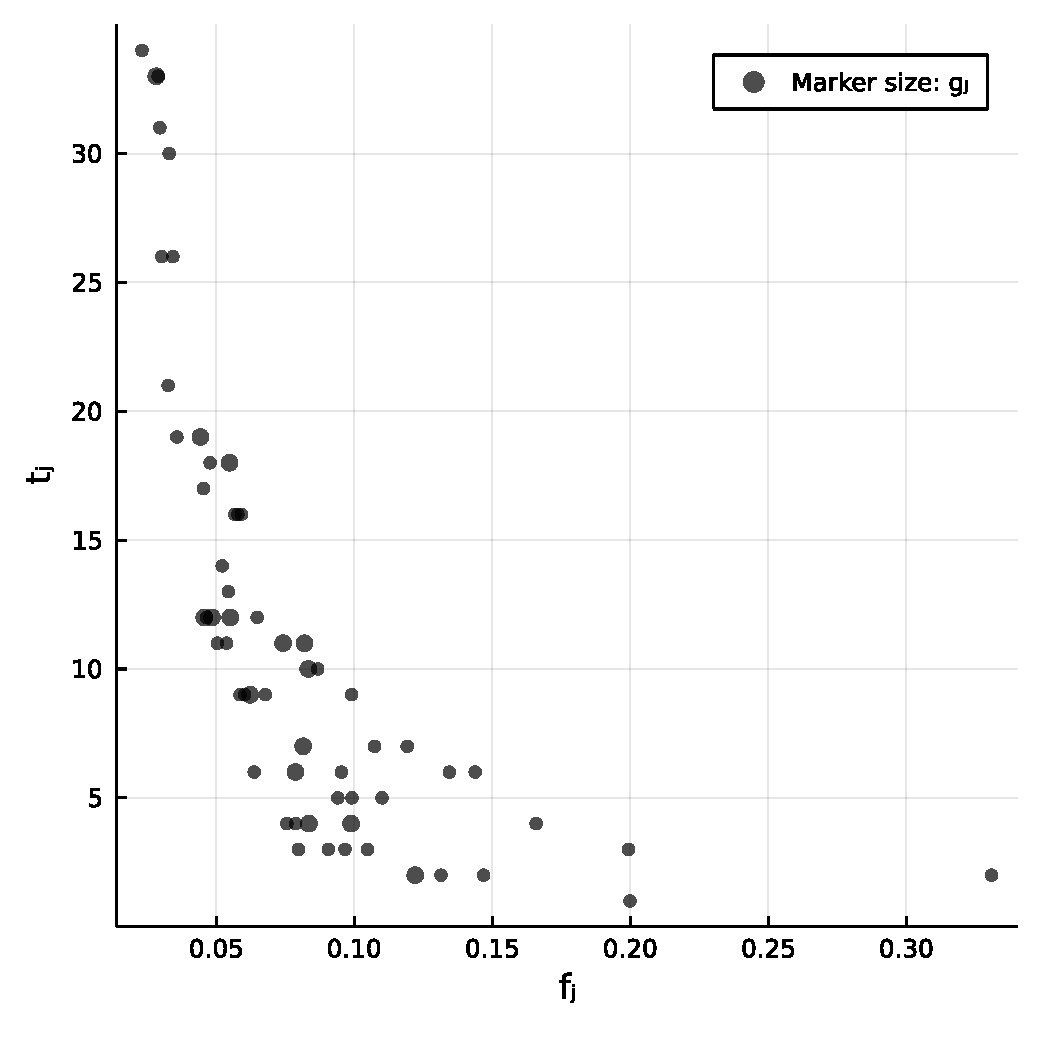
\includegraphics[width=0.75\textwidth]{./plots/samplemarket.pdf}\end{center}
  \caption{A typical randomly-generated instance with $m=60$ schools. }
\end{figure}

The dynamic programs, namely Algorithms \ref{ellisDP1} and \ref{ellisDP3}, were implemented using recursive functions and memoization. Our implementation of Algorithm \ref{ellisDP3} differed slightly from that given above: We represented portfolio valuations in \emph{binary} rather than decimal, with the definitions of $P$ and $\mathcal{V}$ modified accordingly, and instead of fixed-point numbers, we worked in integers by multiplying each $t_j$-value by $2^P$. These modifications yield a substantial performance improvement without changing the fundamental algorithm design or complexity analysis. 



\pagebreak
\ifen \section{Conclusion} \else \section{결론}\fi\label{conclusion}


\pagebreak
\ifen \section{References} \else \section{참고문헌} \fi
\noindent

\parskip 0em
\leftskip 2em
\parindent -2em
\ifen \else
김민희. 2015. ``{[대입 수시 전략]} 총 6번의 기회 \textellipsis `상향·소신·안정' 분산 지원하라.'' 중앙일보, 8월 26일. \url{https://www.joongang.co.kr/article/18524069}.\fi

Budish, Eric. 2011. ``The Combinatorial Assignment Problem: Approximate Competitive Equilibrium from Equal Incomes.'' \emph{Journal of Political Economy} 119 (6): 1061--1103. \url{https://doi.org/10.1086/664613}. 

Dantzig, George B. 1957. ``Discrete-Variable Extremum Problems.'' \emph{Operations Research} 5 (2): 266--88.

\ifen Kim, Minhee. 2015. ``[College application strategy] Six chances total\dots divide applications across reach, target, and safety schools'' (in Korean). Jungang Ilbo, Aug. 26. \url{https://doi.org/10.1086/664613}\fi

Fisher, Marshall, George Nemhauser, and Laurence Wolsey. 1978. ``An analysis of approximations for maximizing submodular set functions—I.'' \emph{Mathematical Programming} 14: 265--94. 

Fredman, Michael Lawrence and Robert Tarjan. 1987. ``Fibonacci heaps and their uses in improved network optimization algorithms.'' \emph{Journal of the Association for Computing Machinery} 34 (3): 596--615.

Fu, Chao. 2014. ``Equilibrium Tuition, Applications, Admissions, and Enrollment in the College Market.'' \emph{Journal of Political Economy} 122 (2): 225--81. \url{https://doi.org/10.1086/675503}. 

Garey, Michael and David Johnson. 1979. \emph{Computers and Intractability: A Guide to the Theory of NP-Completeness.} New York: W. H. Freeman and Company. 

Meucci, Attilio. 2005. \emph{Risk and Asset Allocation.} Berlin: Springer-Verlag, 2005. 

Othman, Abraham, Eric Budish, and Tuomas Sandholm. 2010. ``Finding Approximate Competitive Equilibria: Efficient and Fair
Course Allocation.'' In \emph{Proceedings of 9th International Conference on Autonomous Agents and Multiagent Systems.} New York: ACM. \url{https://dl.acm.org/doi/abs/10.5555/1838206.1838323}.

Rozanov, Mark and Arie Tamir. 2020. ``The nestedness property of the convex ordered median location problem on a tree.'' \emph{Discrete Optimization} 36: 100581. \url{https://doi.org/10.1016/j.disopt.2020.100581}.

% p. 70: FPTAS for knapsack, should work for Ellis's problem
Vazirani, Vijay. 2001. \emph{Approximation Algorithms.} Berlin: Springer. 

\end{document}  

